\section{Problema 1}

\subsection{Enunciado}
El enunciado nos plantea una situación en donde tenemos un edificio con n pisos y personas en cada piso que quiere ir a planta baja. Para poder hacerlo, el edificio provee un 
ascensor que deberá buscar a las personas para poder bajarlas. 
Este ascensor posee energía y capacidad limitada que no le permite recorrer siempre todos los pisos y levantar todas las personas, por lo tanto queremos maximizar la cantidad
de personas a descender del edificio dado la cantidad de personas por piso, su energía y capacidad.

\subsection{Soluci\'on}
La solución planteada utiliza Programación Dinámica a través de decisiones. Planteamos el problema de forma tal que en vez de maximizar la cantidad de personas que 
pueden descender, encontramos el máximo valor posible que va a estar ubicado entre cero y la cantidad de personas totales en el edificio.\\
A continuación se explicará cómo se resolvió el problema:\\
Primero obtendremos la cantidad total de personas recorriendo el edificio dado, y buscaremos el máximo valor de personas que podremos llegar a descender  utilizando la búsqueda binaria entre la cantidad de personas en el edificio, hasta encontrar el valor más alto que se pueda levantar, tal que incrementado en uno no sea posible levantarlo.
En cada paso de la búsqueda binaria, hay que comprobar si se puede levantar cierta cantidad de personas (dada la capacidad del ascensor, su energía y la cantidad de pisos del edificio).
Para comprobar que se puedan levantar buscaremos el piso mínimo al que necesitaremos ir$^*$. Recorreremos el edificio desde el piso mínimo hacia abajo solo en caso de ser posible llegar hasta él y poder volver a descender, levantando la máxima cantidad de personas de cada piso en el camino hasta llenar la capacidad total del ascensor. Una vez completo el ascensor, descenderemos a los pasajeros hasta planta baja y volveremos a repetir el proceso. En el caso de que haya quedado gente y nos quede energía volveremos al mismo piso, en caso contrario seguiremos con el siguiente piso al que podamos ir hasta que levantemos la cantidad requerida o hasta que nos quedemos sin energía (caso que devolveremos que no se puede levantar esa cantidad de gentar). Tener en cuenta que el piso mínimo elegido puede dejarnos en la parte inferior del edificio con más personas de las requeridas. Entonces al momento de levantar puede pasar que no levantemos gente y que sin embargo, descendamos la cantidad requerida de personas.\\
Para la demostración de la resolución explicaremos las razones por las cuales el piso mínimo elegido previamente es el correcto y la estrategia de levantar de arriba hacia abajo es verdadera.
Este piso mínimo es la mejor opción ya que si subimos más pisos estaríamos utilizando energía para levantar la misma cantidad de gente que podríamos encontrar en los pisos
inferiores, y, no se puede ir más abajo porque si no, no tendríamos la cantidad de gente necesaria para poder levantar el valor pedido.\\
Definimos el mundo de las estrategias como el conjunto de estrategias posibles y estrategia como el método por el cual se levanta gente. Como no nos interesa
la energía utilizada, ya que solo queremos ver si puede levantar la cantidad de personas mencionada, y no la optimalidad de energía, una estrategia estará conformada por la cantidad
de personas que el ascensor levanta en cada piso. De este mundo de estrategias tomaremos solo aquellas en las que su piso más alto del cual levantan personas es el nuestro, y que
levanten la misma cantidad que nosotros. Este conjunto es distinto de vacío ya que es un conjunto acotado de personas y pisos, por lo tanto se van a poder levantar a partir de
cierta energía. Ahora queremos ver que nuestra estrategia se encuentra en este conjunto  para lo que tomaremos una de esas estrategias E y veremos que se pueda permutar de tal
forma que consigamos nuestra estrategia. Vamos a dividir a las estrategias verdaderas entre las que levantan mientras suben y el resto.\\
El caso de que E levante mientras sube, ya sabemos que el piso máximo de E es el mismo que 
el nuestro, que podemos ir hasta el piso máximo y al bajar vamos a pasar por los mismos pisos por lo que se terminan levantando la misma cantidad de personas. Puede llenarse antes en los pisos superiores, pero siempre vamos a poder
llenar con los pisos que E llenó.\\
Para el caso desordenado, podremos ubicar la forma que recorre el edificio tal que levante de forma ascendente. Esto sucede ya que si el edificio pasa por los pisos 1 hasta el máximo pero en el medio va agarrando personas en forma desordenada, podemos permutar el método y que vaya levantando mientras asciende. \\
Por lo tanto, tenemos que el segundo caso puede llevarse al primero, y este último hacia el nuestro; y como las estrategias que tomamos son las que funcionaban, entonces la nuestra también funciona.\\

{\footnotesize {\textbf{*} Para ubicar este piso mínimo recorreremos el edificio desde abajo contando la cantidad de personas en los pisos, hasta que el valor sea mayor o igual al requerido.}}

\subsection{Pseudoc\'odigo}
\begin{codebox}
\Procname{$\proc{resolver}$ (\textbf{in} $capacidad$, \textbf{in} $energia$, \textbf{in} $pisos$)}{maximaCantidad}{Int}
\li		totalPersonas = SumaTotalPersonas(pisos);
\li		return BusquedaBinariaPersonas(0,totalPersonas, totalPersonas,energia,capacidad,pisos);
\end{codebox}

\begin{codebox}
\Procname{$\proc{SumaTotalPersonas}$ (\textbf{in} $pisos$)}{acum}{Int}
\li		\textbf{Para} cada piso p \Do
\li			acum = acum + genteEnPiso(p) \End
\end{codebox}

\begin{codebox}
\Procname{$\proc{BusquedaBinariaPersonas}$ (\textbf{in} $desde$, \textbf{in} $hasta$, \textbf{in} $total$,\textbf{in} $energia$, \textbf{in} $capacidad$, \textbf{in} $pisos$)}{acum}{Int}
\li		medio = (desde + hasta)/2;
\li		puedo = sePuedeLevantar(energia, capacidad, pisos, medio);
\li 		\textbf{Si} puedo \Do
\li				\textbf{Si} no se puede levantar el siguiente terminé
\li 				\textbf{Si no} busquedaBinariaPersonas en la siguiente mitad \End
\li 		\textbf{Si no} busquedaBinariaPersonas en la primera mitad
\end{codebox}

\begin{codebox}
\Procname{$\proc{sePuedeLevantar}$ (\textbf{in} $energia$, \textbf{in} $capacidad$, \textbf{in} $pisos$, \textbf{in} $personasABuscar$)}{sePuede}{Boolean}
\li 		\textbf{Para} cada piso empezando desde el piso minimo \Do
\li			\textbf{Si} tengoEnergiaParaLlegar y Hay Gente \Do
\li				\textbf{Si} el piso tiene mas gente que mi capacidad \Do
\li					sumoLoQueLevante
\li					veoSiPuedoVolverAEstePiso \End
\li				\textbf{Si no} \Do
\li					sumoLoQueLevante
\li					mientrasBajoSumoGenteParandoEnLosPisosQueHayGente \End \End
\li			\textbf{Si no} \Do
\li				AnotoLasQueNoLevanté \End \End
\li		return (cuantoLevante >= personasABuscar)
\end{codebox}


\subsection{Analisís de complejidad}	
Para averiguar cuanta gente hay en todo el edificio tenemos que recorrer todo el vector 'pisos' e ir sumando la cantidad de gente en cada piso. Eso nos cuesto O(n) donde n es la cantidad de pisos. Luego hacemos una búsqueda binaria sobre la cantidad total de gente que mediante la función sePuedeLevantar busca el máximo de gente que es posible cargar. La complejidad de la búsqueda binaria es de O(log (cantGente)) (esto es sabido, porque ya fue visto en la materia de Algoritmos y Estructura de Datos II) y la complejidad de la función sePuedeLevantar en el peor caso (sería cuando tiene que irse hasta el último piso para poder levantar la cantidad de gente solicitada y tiene energía suficiente para levantarlos a todos) es de: \\
	O( $\sum\limits_{i=0}^{n} { ( \lceil (pisos[i]/capacidad) \rceil  + i}$ ) ) \\
Esto es porque por cada piso al que voy tengo que ir tantas veces tal que levante el total de gente de ese piso (eso es $\lceil$pisos[i]/capacidad$\rceil$) y luego en caso que me haya sobrado espacio voy recorriendo todos los pisos inferiores para llenar la capacidad restante.
Finalmente la complejidad total del ejercicio nos queda:\\
O( n + Log(g) * $\sum\limits_{i=0}^{n} { ( \lceil (pisos[i]/capacidad) \rceil  + i ) }$ ) \\
Donde n es la cantidad total de pisos y g la cantidad total de gente en todo el edificio.

\subsection{Tests y Gráficos}
En los test quisimos demostrar que cuanto menos capacidad tenga el ascensor (siempre y cuando tenga energía suficiente) mas ciclos va a requerir la resolución. Y por otro lado que la energía es un factor limitante ya que cuanto menos energía tenga el ascensor no solamente va a levantar menos gente sino que ademas va a ciclar menos.
Para los dos gráficos utilizamos el mismo edificio (ya que para lo que queremos demostrar no necesitamos variar el edificio), que es el siguiente: \\

PISO 12 | 45 | \\
PISO 11 | 20 | \\
PISO 10 | 60 | \\
PISO 9  | 90 | \\
PISO 8  | 80 | \\
PISO 7  | 45 | \\
PISO 6  | 8  | \\
PISO 5  | 38 | \\
PISO 4  | 46 | \\
PISO 3  | 66 | \\
PISO 2  | 11 | \\
PISO 1  | 4  | \\

En el siguiente gráfico dejamos fija la energía en un valor muy grande (9700) para que la mimsa no sea un factor limitante.Aquí podemos observar como disminuye la cantidad de ciclos a medida que aumenta la capacidad. Esto es por el factor (pisos[i]/capacidad) que mencionamos en la complejidad, por trivialidad matemática ese factor aumenta a medida q disminuye la capacidad. \\
\begin {center}
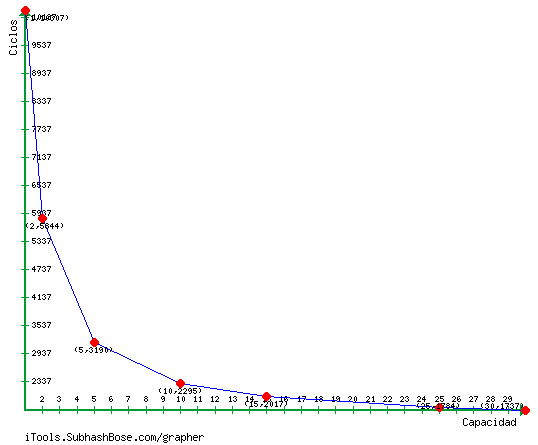
\includegraphics[width=8cm]{./graficos/grafico_ej1_variaCapacidad.png}
% grafico.eps: 0x0 pixel, 300dpi, 0.00x0.00 cm, bb=50 50 410 302
\end {center} 

En el siguiente gráfico dejamos fija la capacidad en un valor chico (5) para demostrar como la energía limita la cantidad de ciclos. Decimos que limita ya que no sólo no nos restringe la cantidad de personas a levantar sino que ademas descartamos muchos casos al resultar imposibles por esta cuestión energética.\\
Claramente podemos observar como los ciclos aumentan al tener mas energía. Notar que también aumenta porque hay mucha gente para levantar y poca capacidad, podría pasar que hubiese un solo piso con 1 persona y en caso, por ejemplo, la energía acotaría muy poco los ciclos, ya que se requieren pocos ciclos para levantar la máxima cantidad de gente.
\begin {center}
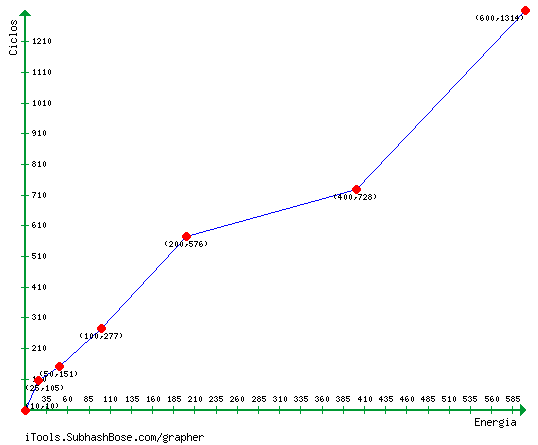
\includegraphics[width=8cm]{./graficos/grafico_variaEnergia.png}
% grafico.eps: 0x0 pixel, 300dpi, 0.00x0.00 cm, bb=50 50 410 302
\end {center} 


\subsection{Conclusiones}
El problema nos mostró que podía ser encarado de distintas maneras dentro de la métodología de programación dinámica. Al principio habíamos utilizado una idea parecida a la de SubSetSum con memorization pero percances en el desarrollo nos hicieron repensar. Por esto, encaramos el problema a través de decisiones lo que nos ayudó a entender el principio de optimalidad.
